\section{Future To Do}

	There is always more to do when it comes to tracking. Improvements to the fitting code, optimization, integration of new features up and down stream, and general code development are a few areas that will require work in the future months and years that this code is in use. Listed here are a few specific sections of work that need to be done, though it is not all inclusive. Some of these sections are hinted at in other parts of this document, some of them are included here as possible sections of work (though not necessarily), and some sections are for work that was started but not completed. These are not ordered in any particular way. (These also might have been taken care of by the time the reader looks through this document.)

	\subsection{Non-Gaussian Garfield Errors}

		When dealing with real data, the errors on the dca measurements that the straws record are non-Gaussian, stemming from the fact that the drift model is non-linear. To align as best we can with real data, James Mott has developed a Garfield model to deal with these measurement attributes, see \href{https://gm2-docdb.fnal.gov/cgi-bin/private/ShowDocument?docid=6171}{DocDB 6171}. However, this still causes trouble for our least squares minimizer since it assumes that the fit errors are Gaussian. If one implements the Garfield model directly in the simulation, then the resultant p-value plot rises at both 0 and 1, see Figure \ref{fig:garfieldPValue}. For this reason these fit errors and their affect on the track fitting need to be studied, understood, and improved where possible, though it is reasonable that their affects are unavoidable.

			\begin{figure}[]
				\caption{Shown here is the p-value distribution for fitted tracks using the Garfield parameterization for the dca errors. It can be seen to spike at 0 and rise towards 1, when in an ideal case it would be uniform, indicating that the fitting is not handling the errors exactly correctly. This is probably unavoidable on some level, but can probably be improved from where it's at now.}
				\centering
				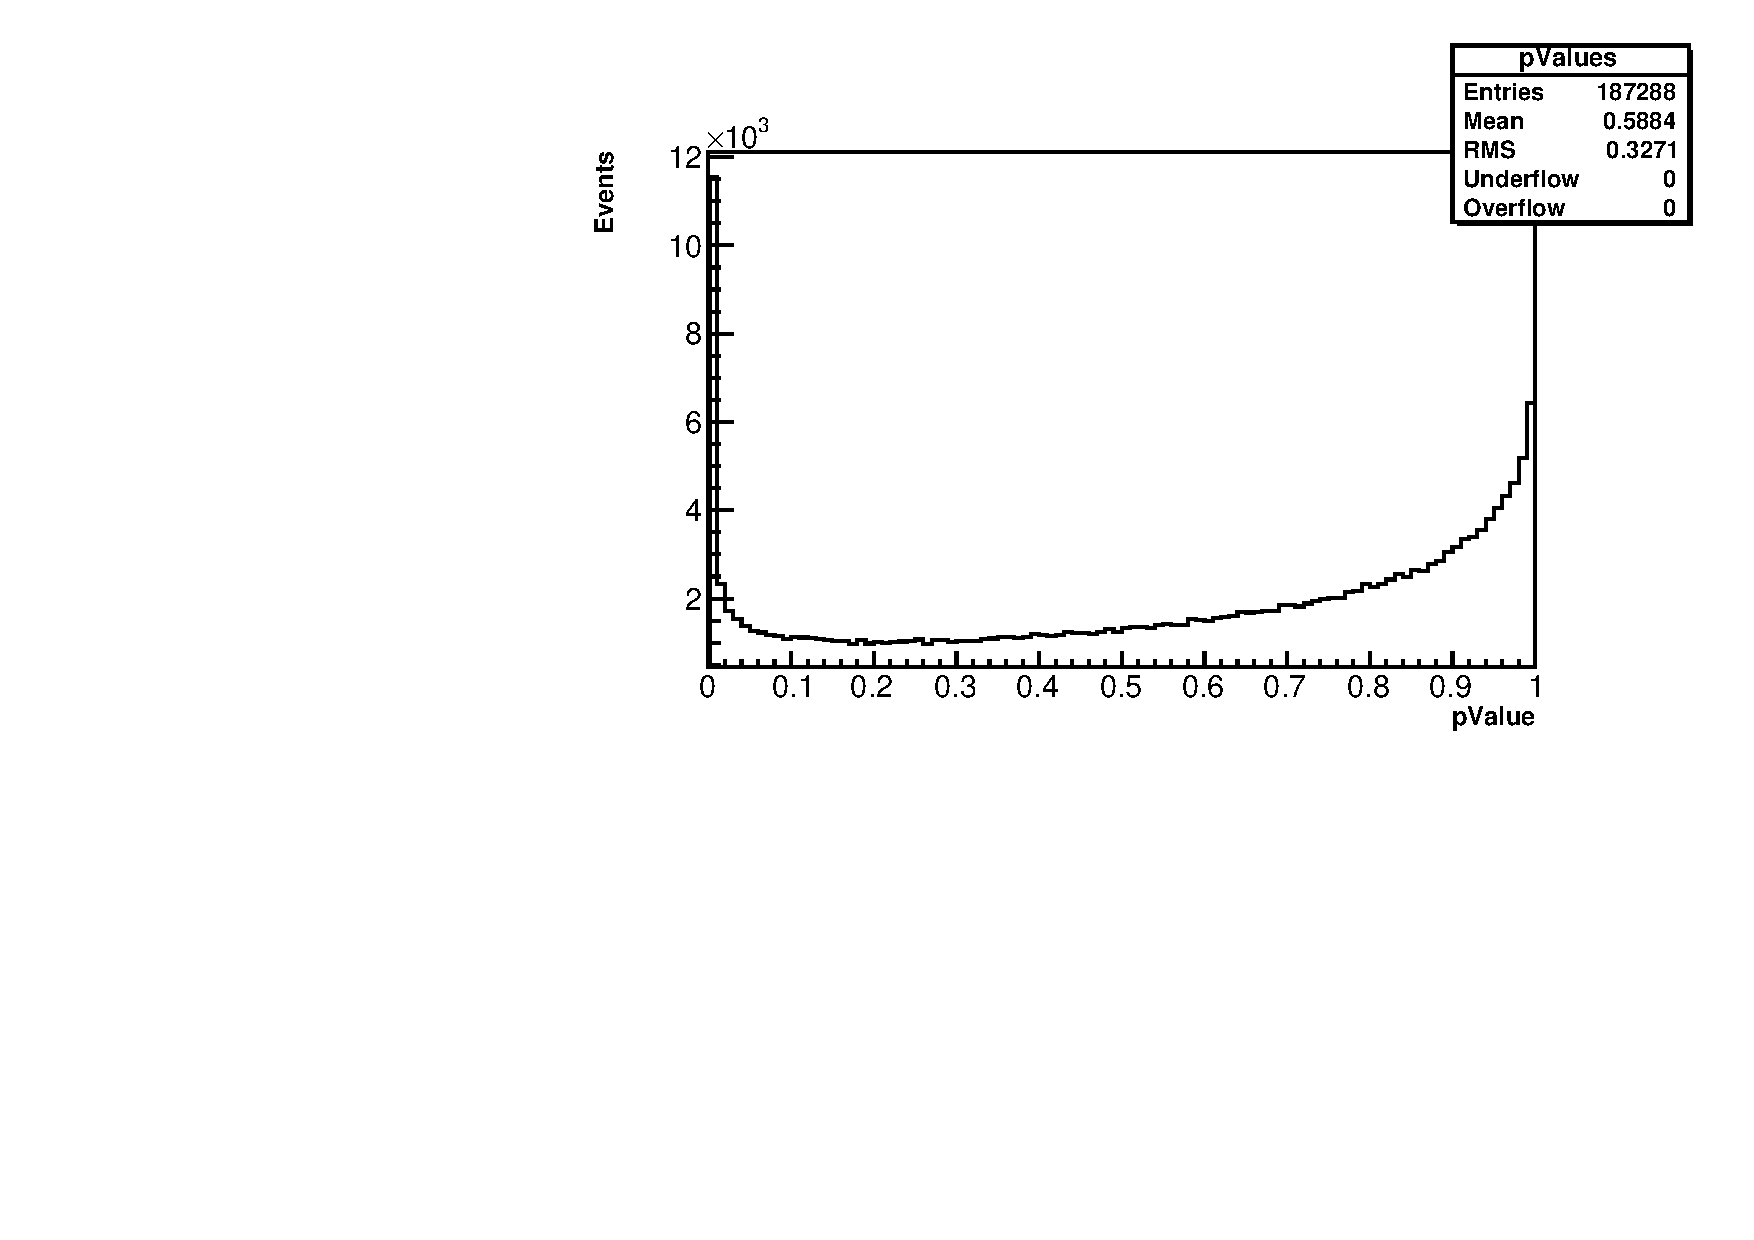
\includegraphics[width=1.0\textwidth]{garfieldPValue}
				\label{fig:garfieldPValue}
			\end{figure}

	\subsection{Measurement pulls on all planes}

		Currently in the track fitting, the measures of how well the track fitting is performing is to look at truth pulls for the parameters on the starting plane as well as the p-value distribution of the fitted tracks. Unit Gaussians for the former and a uniform distribution for the latter prove that the track fitting is working properly. With real data however, the former do not exist, and it is instead more instructive to look at measurement pulls on hit planes. Section 6 of reference \cite{trajfit} has some information on this, with the mathematical form of these measurement pulls defined as:
		\begin{align} \label{eq:measpull}
            \frac{\Delta_{meas}}{\sigma} = \frac{p_{fit} - p_{meas}}{\sqrt{\sigma^{2}_{meas} - \sigma^{2}_{fit}}},
        \end{align}
        where all terms are defined on a single plane.

        However, if these measurement pulls are implemented as in Equation \ref{eq:measpull}, then the resulting distributions are not unit Gaussians as they should be. If I define them as 
        \begin{align} \label{eq:measpullmaterial}
            \frac{\Delta_{meas}}{\sigma} = \frac{p_{fit} - p_{meas}}{\sqrt{\sigma^{2}_{meas} - \sigma^{2}_{fit} + \sigma^{2}_{material}}},
        \end{align}
        where $\sigma_{material}$ is the error due to the material only, then the resulting distributions look more correct. See \href{https://gm2-docdb.fnal.gov/cgi-bin/private/ShowDocument?docid=6261}{DocDB 6261} and \href{https://gm2-docdb.fnal.gov/cgi-bin/private/ShowDocument?docid=6306}{DocDB 6306} for calculations and plots regarding this. The problem however is that this doesn't seem to make a whole lot of conceptual sense, adding this extra error term in. Either this extra term is supposed to be added for reasons not fully understood, or it counteracts some mistake in the measurement pull calculation. Understanding and utilizing this will be necessary when it comes to looking at real data.

	\subsection{Material error tuning}

		While less serious than dealing with the non-Gaussian measurement errors as described above, it will almost certainly be necessary to deal with the material errors as calculated in the Geant4 error propagation routines, specifically the methods ``PropagateErrorMSC'' and ``PropagateErrorIoni'' in the gm2GeaneFreeTrajState.cc file which calculates these material errors. See the \hyperref[sec:gm2Geane]{gm2Geane} section for some more details on this. The reference \cite{Lavezzi} has some sections on the calculation of these errors for the PANDA experiment, and it is readily observed that these calculations differ slightly from those implemented within Geant. This is supposedly because the default Geant calculations are more attuned to denser scatterers, and not PANDA's straw tube tracker which has some resemblance to our straw detectors. This suggests that we should also be making changes. These modifications are currently programmed into that gm2GeaneFreeTrajState.cc file but commented out. Some quick studies with them turned on were done but no real conclusions were made about whether they should be included in our error calculations or not. It is decently likely that some modifications will need to be included in the error calculations, but that they will not be exactly equal to the ones that PANDA used. It is certainly the case that the p-value distribution right now does indeed rise very slightly towards 1, hinting at not-quite-correct error calculation. The measurement pulls can also be a window into the correctness of these error calculations, but first those pulls need to be understood as described above before they are useful.

	\subsection{Starting error/covariance}

		When first creating the free trajectory state for the error propagation, you need to initialize the 5x5 error matrix. For our tracking we've just been using a 0 matrix. That's given us ideal results in a vacuum world, and near ideal results in a material world (with known effects throwing distributions slightly off), indicating that we're performing the track fitting correctly. However it seems like it would make conceptual sense to calculate some error on the track parameters from the initial fitter and use that as an input, as there is an uncertainty in where the track can go that you would want to include.  In the same vein, it seems like it would make sense to use the previous fit iteration covariance matrix as the input error matrix for the next iteration. If any of this is included then the fitting results always worsen however, so they have not been included. This work might be unessecary, but I've included this note just in case.

	\subsection{Initial fitter and effects on Geane fitting}

		For the track fitting, an initial guess for the starting track parameters is needed before doing the Geane fitting. Currently a simple horizontal circle fit to the wire centers is performed upstream in the track finding code. This circle fitter does a remarkably sufficient job for the vast majority of tracks. There are some tracks which do not converge however, and it is possible that this is because the initial fitter is insufficient. That and the fact that the intial fitter was done simply without much thought means that it might be a good place to eek out some better tracking results. General studies on how good this initial fitter needs to be have yet to be completed also, though it's reasonably likely that it's already sufficient. It is also the case that while no biases due to this have been observed with simulated data, they might rear their heads with real data which is something to keep in mind.

	\subsection{Bugs and failed tracks}

		There are always tracks which fail the tracking for one reason or another. See Figure \ref{fig:failureModes}. Some of these are due to unavoidable effects like kinking after interacting with material, and some of these are from very fixable sources. Any tracks which fail due to bugs in the tracking code should absolutely be fixed. Known failures included Geant bugs where the step length is 0 or 1000 mm, a 0 transport matrix is returned in the error propagation stage, the error propagation has gotten past the target, or the error propagation returns an internal failure. The exact sources of these bugs are difficult to determine considering that its Geant source code where the problems lie. Some tracks also begin error propagation within the material G4\_AIR, and those have been marked to fail. This might be occuring because the intial fitter does so poor of a job that the track starts outside the storage region, or something more sinister might be going on. There is also a bug where in a vacuum world some tracks experience physical processes like ionization or bremmstrahlung (\href{https://gm2-docdb.fnal.gov/cgi-bin/private/ShowDocument?docid=6183}{DocDB 6183}), which causes some simulated tracks to reconstruct poorly (though not necessarily fail directly). James Stapelton will at some point look more into this since it has some deeper Geant source, but it's good to keep in mind.

		There are still some tracks however that return negative or nan $\chi^{2}$s which have unknown sources. These combined with tracks that diverge leaves a set of tracks that while small are the most important to really understand and fix wherever possible. The latter can probably be improved with a better initial fitter though not fully removed. (There are also some tracks which don't diverge, but also don't converge with a very small $\Delta\chi^{2}$ between iterations, though these are technically not designated as failures.) Finally there are sources of failures from the upstream tracking code. While most such problems have been fixed, there remains the tracks which end up with more than one digit on a single layer, which the Geane fitting cannot handle. It is also very likely that more unseen issues exist since this is a very complicated chain of track reconstruction.

		With further development of the tracking code, both locally, in the upstream reconstruction chain, or even the greater surrounding framework, more bugs or failed tracks will arise. Such new bugs will usually manifest themselves in tracks with negative or nan $\chi^{2}$s, so if the number of such tracks increases then once can be reasonably sure that a new problem has arisen. This is natural and unavoidable, and it is simply a matter of fixing these issues as they appear. Similarly, as data comes in there is a good chance that new failures will appear, which could possibly be due to more subtle issues. (Though I should mention that no such things were seen with the wire fits on the commissioning data.)

	\subsection{Physical processes and kinked tracks}

		As detailed in the \hyperref[sec:AnaFilt]{Analyzers and Filters} section, there is some code that has been partially written regarding the physical processes that the simulated tracks undergo. It would be a good idea to really undertand the effects on the track fitting due to these physical processes. There is a little bit of information on this in \href{https://gm2-docdb.fnal.gov/cgi-bin/private/ShowDocument?docid=6099}{DocDB 6099}. It is certainly the case that because the Geane fitting creates average trajectory states and adds the error due to material, most tracks are properly treated, but there are some tracks which kink or lose a larger amount of energy and fit poorly. These can usually (but not always) be removed from the tracking results with an energy cut for simulated events. For real data however these effects will still exist. Understanding them and reducing them until they are irreducible will be a necessary step before really looking at all the tracks from data. Certainly for kinked tracks, it should be possible to identify them with some smarter criteria in the analyzer stage other than just looking at event displays as in Figure \ref{fig:Kink}. There is some unfinished code (with some sort of unknown issues) in the GeanePlots module which looks at the TrajectoryArtRecords for this reason, which has been left in for the future.

			\begin{figure}[]
				\caption{Shown here is a position plot from the GeaneSingleEventViewer analyzer. The black dots on the red line indicate the true positions of the track that is being reconstructed, with the red line simply connecting the dots. The black line and dots indicates the reconstructed track and positions. The view is side on, with the X axis being the X position of the hits in the reconstruction frame, with particle direction going from left to right as particles pass through the different straw layers. The Y axis indicates the Y position of the track. It can be seen that the true track has upward momentum at the start, hits some material, and kinks at about -1440 mm. (It starts curving back upwards further on because this track was located in a region with some radial field component.) The Geane fitting does it's best to form an average reconstructed track which is seen to be a smooth approximation to the kinked track. This will of course result in a fit with a large $\chi^{2}$.}
				\centering
				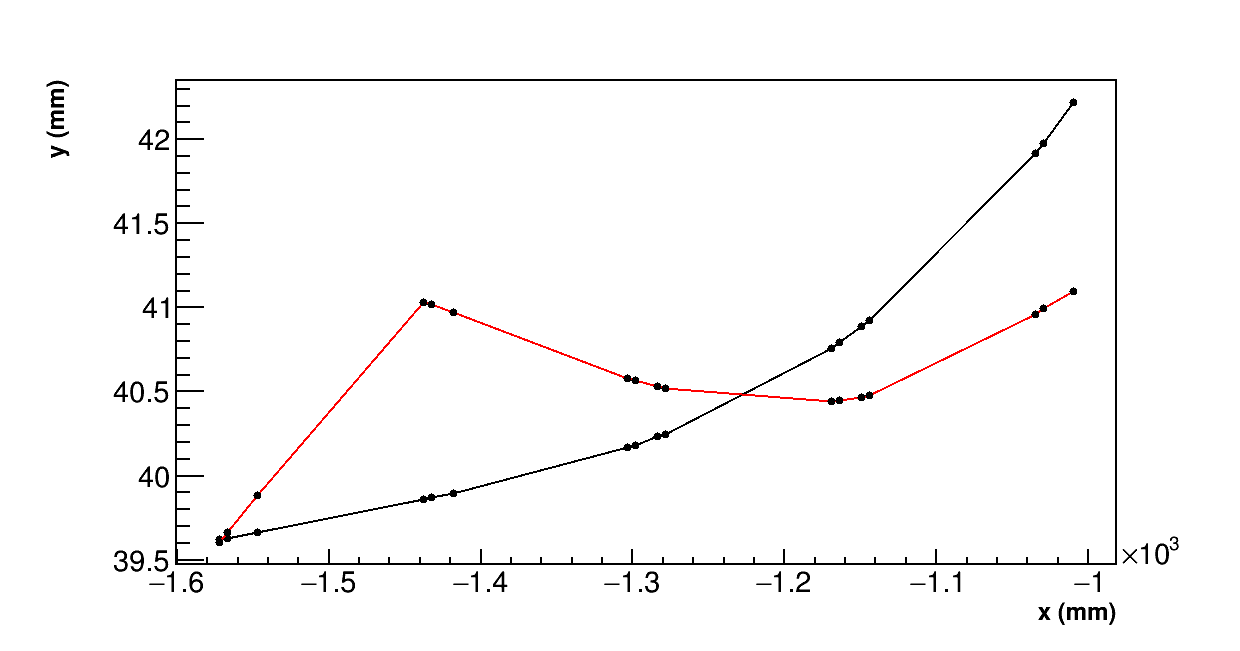
\includegraphics[width=1.0\textwidth]{Kink}
				\label{fig:Kink}
			\end{figure}

	\subsection{Tracker alignment geometry and magnetic fields}

		Currently in the simulation and reconstruction all trackers have the same perfect placed geometry with wire planes exactly parallel to one another. In reality the different trackers will have slightly different geometry due to imperfect placement into the vacuum chambers as well as slight wire warping. See Figure \ref{fig:Alignment}. Once the alignment is completed as best it can be, both physically improved and misalignments recorded (Gleb Lukicov and others), the resultant geometry differences should be coded up and included for the best results possible. It's not clear to me exactly what this will entail, or what complications in the fitting will arise but it should be kept in mind. Certainly the track fitting results without this are worse since the Geane fitting assumes parallel measurement planes, which is not quite the case.

			\begin{figure}[]
				\caption{Shown here is a toy model of the alignment code being developed by Gleb Lukicov. The circles represent the straws with the shaded circles being the hits. In the upper picture an exaggerated vertical misalignment in the two center modules can be seen, with the lower picture being the ideal geometry. In red are the straight line fitted tracks to the hit straws. It can be seen that the misalignment in the top picture produces tracks which differ from the true tracks in the lower picture. This means that without the alignment included in the reconstruction we will reconstruct tracks with an excluded error.}
				\centering
				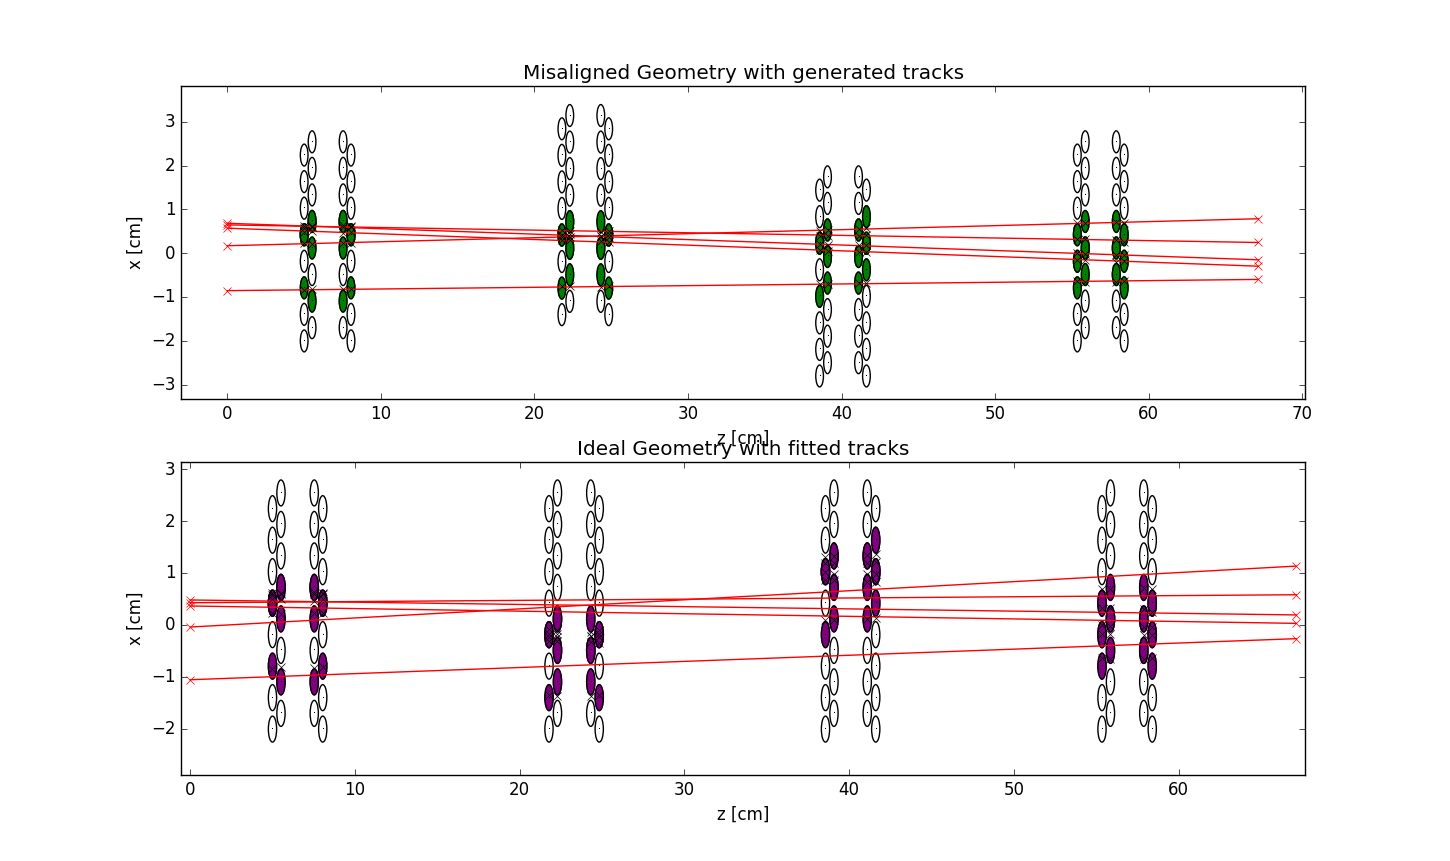
\includegraphics[width=1.0\textwidth]{Alignment}
				\label{fig:Alignment}
			\end{figure}

		In a similar vein, the current track fitting incorporates an azimuthally symmetic 2D magnetic field when fitting tracks for the different trackers. This ignores the full 3D field and any differences between the trackers. (Eg. There is no radial field in the simulation currently.) The effects might be negligible, or it might be necessary to include these differences for proper tracking results. It should be on others to calculate, measure, and add these fields to the gm2 simulation, but it will be necessary to update the field setting code in GeaneParamUtils.cc to implement them in the fitting.

	\subsection{Small dcas}

		As seen in \href{https://gm2-docdb.fnal.gov/cgi-bin/private/ShowDocument?docid=6171}{DocDB 6171} the uncertainty in the dca value measured in a straw when a particle passes close to the wire ($\textless{}500 \mu m$) is large. For this reason such measurements will be set to the wire center with a larger error. There is code available to do this as described in the \hyperref[sec:GeaneLRUtils]{GeaneLRUtils} section, which has been shown to work. However, exactly what this threshold should be set at, and its combination with the Garfield errors as described above have yet to be implemented. It's important to do this right for correct tracking results, as even a single measurement in a track with incorrectly assigned errors can throw the whole track off.

	\subsection{5x5 fitter}

		Deepak Sathyan has created the 5x5 fitter as detailed in the Geane manual, as opposed to my more complex full fitter which includes the material correlations. The first results from it are shown in \href{https://gm2-docdb.fnal.gov/cgi-bin/private/ShowDocument?docid=6950}{DocDB 6950} though improvements have been made since then. It can be seen that the results are actually very similar to those from the full fitter. The code itself lives in Deepak's repository on the gm2 machines, and has not been officially added to the feature/trackDevelop branch of the git repository. For speed reasons it will be a good idea to perform the first iterations of the track fitting with this 5x5 fitter which is faster than the full fitter, and only use the full fitter for the laster iteration or so. This should speed up the code significantly without harming physics results.

	\subsection{Commissioning data}

		The June 2017 commissioning run for Muon g-2 gathered some very useful data for the trackers. Some of the data and resulting fitted tracks are detailed in \href{https://gm2-docdb.fnal.gov/cgi-bin/private/ShowDocument?docid=6992}{DocDB 6992}, \href{https://gm2-docdb.fnal.gov/cgi-bin/private/ShowDocument?docid=7463}{DocDB 7463}, and \href{https://gm2-docdb.fnal.gov/cgi-bin/private/ShowDocument?docid=7571}{DocDB 7571}. While there is an extent to the usefulness of the data gathered during the commissioning run due to the prevalence of protons, and there is a wealth of work that needs to be done to improve the tracking, it would still be beneficial to examine the commissioning data more thoroughly. Doing so could reveal features that the data exhibits that simulation does not, point to bugs or insufficiencies in the tracking code, teach about the tracking in general, etc. Certainly examining this data will be a nice preparation for the data that will come in starting in November and beyond.

	\subsection{Further left-right work}

		As detailed in the \hyperref[sec:GeaneLRUtils]{GeaneLRUtils} and \hyperref[sec:LR]{Left-Right} sections a good amount of work has been done regarding handling the left-right ambiguities of the straw measurements within the track fitting. However this code can certainly be expanded and improved to deal with this better and faster. When updates to the track finding code have been made upstream to help deal with this left-right problem, those updates also need to be integrated with the local Geane fitting code. Further studies beyond \href{https://gm2-docdb.fnal.gov/cgi-bin/private/ShowDocument?docid=6800}{DocDB 6800} should also be conducted in order to optimize the tracking results vs speed.

	\subsection{Refinement}

		At the time of writing this, the ``Refinement'' stage of the track reconstruction has not been started. This refinement stage has the job of refining the track by adding hits, removing hits, updating errors, making improvements to left-right guesses, updating T0, and more. While not a direct part of the Geane fitting code, this stage will take information from the Geane fitting results, do its work, and then loop back and refit the track. For this reason, there will be a great deal of work that needs to be done regarding this refinement stage in the future. Be aware that this work will take a very long time (both the updates to the local Geane fitting code and the general refinement stage coding), probably on the order of a year or more, but is a necessary addition to the whole track reconstruction.

	\subsection{Short track fitter}

		Tracks which hit a smaller number of planes naturally fit worse with greater uncertainty on the fitted track. There is a hard cutoff in the upstream reconstruction chain at 6 planes hit. There is a noticeable difference in the fit of tracks that hit 7 or 8 planes vs 9 or more. This is because tracks that hit 7 or 8 planes in adjacent modules have a smaller track length which makes fitting the momentum more difficult. However if those 7 or 8 planes are spread out among modules separated by larger distances then the fit can still be good. This is something to be kept in mind when looking at fitting results.

		For tracks with 6 or less planes hit however, the hard cutoff has been in place since the development of the Geane fitting code. Because a good number of muons will decay close to the calorimeter and curve sharply through 6 or less planes it will be necessary to be able to fit these ``short'' tracks. The Geane fitting code should technically be able to handle these short tracks, though the results will certainly be worse, and this needs to be studied. Separately, and maybe with more priority, a specialized short track fitter will probably need to be written.

	\subsection{Geane extrapolation}

		After the track fitting stage comes the extrapolation stage, where the fitted track is extrapolated back into the storage region in order to determine the muon beam profile. Saskia Charity has developed the extrapolation code that we've been using. With the goal of having more than one version of every stage of the track reconstruction code however, we'll need a second track extrapolator at some point. The Geant4 Geane error propagation routines provide a nice and straightforward way to do this, which is why I've included a note about it here even though it is not directly related to the Geane fitting. One can pull out and modify the relevant code described in the \hyperref[sec:GeaneParamUtils]{GeaneParamUtils} file to do this. Deepak Sathyan has started this but it requires more work going forward.

	\subsection{Optimization}

		While mentioned in the intro to this section, I thought I'd quickly mention optimization. The Geane fitting code like all others needs to be optimized in pretty much all ways. Memory and speed can certainly be improved, maybe even by an order of magnitude or so. I have done very little work regarding this part of the code. Deepak Sathyan quickly and easily improved the track fitting speed by 5x, the first results of which are shown in \href{https://gm2-docdb.fnal.gov/cgi-bin/private/ShowDocument?docid=7094}{DocDB 7094}. More can and needs to be done.

	\subsection{Miscellaneous}

		I'll mention a couple smaller pieces of work here that shouldn't be forgotten.

		In the track fitting, the tungsten wires within the gas should be removed (and just replaced with gas). Due to the uncertainty in the fitted track, it isn't clear whether the track would have gone through a wire or not. If it does in the error propagation however, then a large number is added to the error due to passing through the tungsten material, which is not something we want to include.

		When completing wire fits (very useful for data), there is a discreteness to the results since there is only so many combinations of wires that can be hit. (And a set of hit wires will reconstruct exactly the same track for a wire fit.)  This discreteness and its effects should probably be studied in a little more detail, as they seem to introduce some slightly weird effects in the tracking results, as shown in \href{https://gm2-docdb.fnal.gov/cgi-bin/private/ShowDocument?docid=7463}{DocDB 7463}. Not only that but its possible that this discreteness might be taken advantage of by using some sort of quick look up table to shortcut the wire fit for a known set of wires, per James Mott's suggestion.


